\documentclass{article}
\usepackage[utf8]{inputenc}
\usepackage{polski}
\usepackage{amsmath,amssymb,graphicx,subfig,pdfpages,enumitem,empheq,verbatim,csvsimple}
\usepackage{multirow}

\author{Krystian Baran 145000}
\title{Kolokwium zaliczeniowe nr. 2}

\begin{document}

\maketitle
\newpage

\tableofcontents
\newpage

\section{Zadanie 1}
\textbf{Zadanie 1 (15).} Stosowane w konstrukcjach budowlanych liny stalowe produkowane są trzema
technologiami. Przedmiotem badania są wytrzymałości na rozciąganie $W_1$, $W_2$, $W_3$ tych lin
mierzone w $kG/cm^2$. W tym celu przeprowadzone zostały dla nich badania wytrzymałościowe
i uzyskano następujące wyniki: \\

Dla lin produkowanych pierwszą technologią: 999, 1025, 982, 959, 996, 946, 1041, 1138, 1034,
958, 1039, 1038, 995, 1099, 886, 1064, 1038, 1005, 1010, 1020, 1126, 992, 1029, 1060, 957,
980, 1057, 1037, 891, 923, 1064, 965, 910, 906, 1013, 829, 1066, 1006, 955, 992. \\

Dla lin produkowanych drugą technologią: 944, 982, 919, 886, 940, 867, 1005, 1148, 995, 883,
1003, 1001, 938, 1090, 779, 1039, 1001, 953, 960, 975. \\

Dla lin produkowanych trzecią technologią: 967, 861, 980, 1034, 1045, 925, 991, 920, 958,
1004, 949, 975, 932, 909, 946, 896, 991, 1088, 984, 908, 989, 988, 945, 1049, 836, 1014, 988,
955, 960, 970, 1076, 942, 979, 1010, 907, 930, 1007, 987, 841, 873, 779, 1016, 956, 905, 942,
1014, 915, 860, 856, 963. \\

\textbf{Polecenia:}
\begin{enumerate}[label = \alph*)]
\item Przeprowadzić testy losowości danych pomiarowych.
\item Oceniając skośność oraz kurtozę dokonać wstępnej oceny rozkładów wytrzymałości
i na tej podstawie wskazać rodziny rozkładów, do których mogą należeć badane
wytrzymałości lin.
\item Przeprowadzając odpowiednie testy dokonać identyfikacji rozkładów wytrzymałości
lin dla poszczególnych technologii. Uzasadnić wybory zastosowanych testów.
\item Przyjmując poziom ufności 0,9 wyznaczyć minimalną wielkość próby potrzebną do
oszacowania oczekiwanej wytrzymałości lin produkowanych drugą technologią
z dopuszczalnym błędem maksymalnym 20 $kG/cm^2$.
\item Wyznaczyć 95-procentowe prawostronne przedziały ufności dla przeciętnych
wytrzymałości lin produkowanych poszczególnymi technologiami. Uzasadnić wybór
konstrukcji przedziału.
\item Wyznaczyć 95-procentowe dwustronne przedziały ufności dla odchyleń standardowych
wytrzymałości lin produkowanych poszczególnymi technologiami.
\item W pewnych zastosowaniach budowlanych norma wytrzymałości lin wynosi 865 $kG/cm^2$. Dla lin produkowanych trzecią technologią wyznaczyć 95-procentowy
prawostronny przedział ufności dla wskaźnika lin nadających się do tego zastosowania.
W przypadku niespełniania odpowiedniego założenia zdublować wszystkie dane.
\item Dla wytrzymałości lin produkowanych pierwszą i trzecią technologią sprawdzić, czy
odchylenia standardowe $\sigma_1$ i $\sigma_3$ istotnie różnią się.
\item Dla wytrzymałości lin produkowanych pierwszą i drugą technologią sprawdzić hipotezę $\sigma_1^2 = 0,5 \sigma_2^2$.
\item Przyjmując, że hipoteza $\sigma_1^2 = 0,5 \sigma_2^2$
jest prawdziwa sprawdzić hipotezę $m_1 - m_2 = 50$, gdzie $m_1$, $m_2$ są oczekiwanymi wytrzymałościami lin produkowanych pierwszą
i drugą technologią.
\item Na poziomie istotności 0,05 sprawdzić hipotezę, że wytrzymałość lin produkowanych
pierwszą technologią jest istotnie większa od wytrzymałości lin produkowanych trzecią
technologią.
\item Przeprowadzić testy równości wariancji wytrzymałości lin produkowanych trzema
technologiami.
\item Wygenerować próbę o liczebności $n_4 = 80$ wytrzymałości $W_4 \sim N(1000; 65)$ z kodem
złożonym z pięciu lub czterech cyfr numeru legitymacji studenckiej. Następnie na
podstawie danych dotyczących $W_1$, $W_3$, $W_4$ przeprowadzić analizę wariancji. 
\end{enumerate}

% Punkt A
\subsection{a)}
Jako test losowości próby zastosujemy test Walda Wolfowitza. W pakiecie "randtests" w R istnieje funkcja wykonująca taki test, zatem nie musimy obliczać wartości pośrednie. Jest to funkcja \textit{runs.test()}. Funkcja ta oddała następujące wartości które zostały zebrane w tabeli.
\begin{center} \begin{tabular}{|c|c|c|c|c|c|c|} \hline
Lina & statistic & runs & n1 & n2 & n & p-value \\ \hline
$W_1$ & 0.64072 & 23 & 20 & 20 & 40 & 0.5217 \\ \hline
$W_2$ & 0.45947 & 12 & 10 & 10 & 20 & 0.6459 \\ \hline
$W_3$ & 0.85732 & 29 & 25 & 25 & 50 & 0.3913 \\ \hline
\end{tabular} \end{center}
"statistic" to wartość statystyki testowej, "runs" to ile razy zmienił się znak ponieważ z ciągu liczb przekształcamy na ciąg "+" i "-", "n1" to liczba znaków "+" lub "-", "n2" to liczba znaków przeciwna do znaku liczb z "n1", "n" to całkowita liczebność próby, "p-value" to interesowana nas wartość do porównania z poziomem istotności który przyjmiemy $\alpha = 0.05$. Widzimy że każde \textit{p-value} jest od poziomu istotności większe, a zatem nie możemy odrzucić hipotezę zerową mówiącą że dane pochodzą z losowej próby.

 % Punkt B
\subsection{b)}
Za pomocą funkcji w R obliczono skośność \textit{skewness} i kurtozę \textit{kurtosis}; uzyskano następujące dane dla każdego zestawu:
\begin{center} \begin{tabular}{|c|c|c|} \hline
Lina & skośność & kurtoza \\ \hline
$W_1$ & -0.3325828 & 3.229922 \\ \hline
$W_2$ & 0.002122275 & 3.694011 \\ \hline
$W_3$ & -0.385574 & 3.210685 \\ \hline
\end{tabular} \end{center}

$W_1$ i $W_3$ mają ujemną skośność co oznacza że rozkład może być typu Weibulla z odpowiednio dobranym parametrem lub rozkład minimum Gumbela. Natomiast $W_2$ ponieważ ma skośność w aproksymacji równą 0 i dodatnią kurtozę to może to być rozkład normalny, lub, nie aproksymując skośność do 0, rozkład logarytmiczno-normalny, maksymalnego Gumbela, gamma lub Weibulla; najbardziej prawdopodobne jest rozkład normalny dal tych danych.

% Punkt C
\subsection{c)}
Po przeprowadzeniu wstępnej analizy skośności i kurtozy możemy przeprowadzić testy zgodności z danym rozkładem aby sprawdzić czy dane mają jeden z wymienionych wcześniej rozkładów. Zastosujemy test Kołmogorowa Smirnova dostępny w R pod \textit{ks.test()}. Aby sprawdzić zgodność z danym rozkładem parametry tego rozkładu estymowano funkcją \textit{fitdistr()}. \\

Dla $W_1$ testowano zgodność z rozkładem Weibulla i normalnym. Wartosci oddane przez \textit{fitdistr()} i  podane poniżej:
\begin{center} \begin{tabular}{|c|c|c|c|c|} \hline
& \multicolumn{2}{|c|}{fitdistr} & \multicolumn{2}{|c|}{ks.test} \\ \hline
Rozklad & shape & scale & D & p-value \\ \hline
Weibull & 17.276191 & 1030.197109 & 0.10195 & 0.8 \\ \hline
& mean & sd & & \\ \hline
Normal & 1000.750000 & 64.078760 & 0.095693 & 0.8573 \\ \hline
\end{tabular} \end{center}
Ponieważ \textit{p-value} jest większe niż poziom istotności $\alpha = 0.05$ nie możemy odrzucić hipotezę o równaniu się temu rozkładowi. Zatem dane mogą pochodzić z rozkładu Weibulla lub z rozkładu normalnego. \\ \par

Dla $W_2$ testowano zgodność z rozkładem normalnym, Weibulla, logarytmiczno-normalny i gamma. Użyto te same funkcje co poprzednio i otrzymano wartości podane poniżej. \\
Normalny : mean  = 965.40000,  sd = 78.34437 \\
Weibulla : shape = 12.630921, scale = 1001.631919 \\ 
Gamma : shape = 144.2522661, rate = 0.1494225 \\
Lognormal : meanlog = 6.86920904, sdlog = 0.08200440

\begin{center} \begin{tabular}{|c|c|c|} \hline
Rozkład & D & p-value \\ \hline
Normalny & 0.15662 & 0.7105 \\ \hline
Weibulla & 0.20229 & 0.3863 \\ \hline
Gamma & 0.15371 & 0.7321 \\ \hline
Lognormal & 0.14775 & 0.7751 \\ \hline
\end{tabular} \end{center}
Porównując \textit{p-value} z przyjętym poziomem istotności $\alpha = 0.05$ widzimy że nie możemy odrzucić żadną hipotezę zerową równania się rozkładów. Natomiast, porównując otrzymane wartości, widzimy że najmniejsza jest dla rozkładu Weibulla, co oznacza że dane te najmniej prawdopodobnie pochodzą z rozkładu Weibulla. \\ \par

Dla $W_3$ także przeprowadzono test dla rozkładu Weibulla i normalnym jak dla poprzednich danych. Otrzymane wartości zapisano poniżej:
\begin{center} \begin{tabular}{|c|c|c|c|c|} \hline
& \multicolumn{2}{|c|}{fitdistr} & \multicolumn{2}{|c|}{ks.test} \\ \hline
Rozklad & shape & scale & D & p-value \\ \hline
Weibull & 17.177821 & 982.722097 & 0.095061 & 0.7569 \\ \hline
& mean & sd & & \\ \hline
Normal & 954.300000 & 62.404888 & 0.081875 & 0.8909 \\ \hline
\end{tabular} \end{center}
Obliczone \textit{p-value} jest większe od przyjętego poziomu istotności $\alpha = 0.05$ zatem nie możemy odrzucić hipotezę zerową że dane pochodzą z rozkłady Weibulla tak jak i z rozkładu normalnego.

% Punkt D
\subsection{d)}
Ponieważ dane z drugiej metody są z dużym prawdopodobieństwem normalnie rozłożone a nie znamy wartości oczekiwanej ani wariancji tego rozkładu, możemy zastosować poniższy wzór na obliczenie minimalnej liczebności próby.
\[ n = \Big \lceil \frac{t_{1 - \frac{\alpha}{2}; n_0 - 1}^2 S_{n_0}^2}{d^2} \Big \rceil \]
Gdzie $d = 20$ jest maksymalny błąd, $n_0 = 20$ to liczebność próby, $1 - \alpha = 0.9 \rightarrow \alpha = 0.1$
\[ S_{n_0}^2 \overset{R}{=} var(w2) = 6460.884 \]
\[ t_{1 - \frac{\alpha}{2}; n_0 - 1} \overset{R}{=} qt(0.95, 19) = 1.729133 \]
Podstawiając do wzoru otrzymujemy: 
\[ n = \Big \lceil \frac{1.729133^2 \cdot 6460.884}{20^2} \Big \rceil = \lceil 48.292507 \rceil = 49 \]
Zatem, minimalna próba żeby na poziomie ufności 0.9 i z błędem maksymalnym 20 $kG/cm^2$ wyznaczyć wartość oczekiwaną jest 49.

% Punkt E
\subsection{e)}
Aby wyznaczyć przedział ufności na poziome ufności $1 - \alpha = 0.95$ potrzebujemy rozważyć dane. Dla $W_1$ i $W_3$ nie przyjmujemy że to rozkład normalny, natomiast liczebność jest na tyle wielka że można zastosować poniższy wzór na prawostronny przedział ufności.
\[ ( \overline{W} - z_{1 - \alpha} \frac{S_n}{\sqrt{n}} , \infty ) \]
Gdzie:
\[ z_{1 - \alpha} \overset{R}{=} qnorm(0.95, 0, 1) \approx 1.644854 \]
\begin{center} \begin{tabular}{|c|c|c|c|} \hline
Lina & $\overline{W}$ & $S_n^2$ & $S_n$ \\ \hline
$W_1$ & 1000.75 & 4211.372 & 64.89508 \\ \hline
$W_2$ & 965.4 & 6460.884 & 80.37963 \\ \hline
$W_3$ & 954.3 & 3973.847 & 63.03846 \\ \hline
\end{tabular} \end{center}

Zatem dla $W_1$:
\[ 1000.75 - 1.644854 \frac{64.89508}{\sqrt{40}} \approx 983.872461 \]
\[ ( 983.872461 ; \infty ) \]
Dla $W_3$:
\[ 954.3 - 1.644854 \frac{63.03846}{\sqrt{50}} \approx 939.636152 \]
\[ ( 939.636152 ; \infty ) \]

Dla $W_2$, ponieważ nie odrzuciliśmy hipotezę o równości z rozkładem normalnym, możemy zastosować następujący wzór na przedział ufności:
\[ ( \overline{W} - t_{1 - \alpha; n-1} \frac{S_n}{\sqrt{n}} , \infty ) \]
\[ t_{1 - \alpha; n-1} \overset{R}{=} qt(0.95, 19) \approx 1.729133 \]
Zatem
\[ 965.4 - 1.729133 \frac{80.37963}{\sqrt{20}} \approx 934.321546 \]
\[ ( 934.321546 ; \infty ) \]

% Punkt F
\subsection{f)}
Ponieważ przeprowadziliśmy test równości z rozkładem normalny i nie uzyskaliśmy sprzecznego wyniku możemy dla każdego zestawu danych wyznaczyć dwustronny przedział ufności. Natomiast, dla $W_2$, sokoro mamy mniej niż 20 elementów to zastosujemy inna konstrukcje jak dla $W_1$ i $W_3$. \\
Dla $W_1$ i $W_3$ wzór na przedział będzie następujący, gdzie badane jest odchylenie standardowe:
\[ \Big( \frac{\sqrt{\frac{n-1}{n}} S_n}{1 + \frac{z_{1-\frac{\alpha}{2}}}{\sqrt{2n}} } ; \frac{\sqrt{\frac{n-1}{n}} S_n}{1 - \frac{z_{1-\frac{\alpha}{2}}}{\sqrt{2n}} } \Big) \]
Gdzie
\[ z_{1-\frac{\alpha}{2}} \overset{R}{=} qnorm(0.975, 0, 1) \approx 1.959964 \]
Zatem dla $W_1$ przedział wygląda następująco:
\begin{align*}
\Big( \frac{\sqrt{\frac{39}{40}} \cdot 64.89508}{1 + \frac{1.959964}{\sqrt{80}} } & ; \frac{\sqrt{\frac{39}{40}} \cdot 64.89508}{1 - \frac{1.959964}{\sqrt{80}} } \Big) \\
( 52.561026 &; 82.06079 )
\end{align*}

Dla $W_3$ przedział będzie wyglądać następująco:
\begin{align*}
\Big( \frac{\sqrt{\frac{49}{50}} \cdot 63.03846}{1 + \frac{1.959964}{\sqrt{100}} } & ; \frac{\sqrt{\frac{49}{50}} \cdot 63.03846}{1 - \frac{1.959964}{\sqrt{100}} } \Big) \\
( 53.714921 &; 79.903686 )
\end{align*}

Dla $W_2$ wzór będzie następujący gdzie badana jest wariancja zamiast odchylenia standardowego
\[ \Big( \frac{(n-1)S_n^2}{\chi^2_{1-\frac{\alpha}{2};n-1}} ; \frac{(n-1)S_n^2}{\chi^2_{\frac{\alpha}{2};n-1}} \Big) \]
Gdzie
\[ \chi^2_{1-\frac{\alpha}{2};n-1} \overset{R}{=} qchisq(0.975, 19) \approx 32.85233 \]
\[ \chi^2_{\frac{\alpha}{2};n-1} \overset{R}{=} qchisq(0.025, 19) \approx 8.906516 \]
Zatem przedział ufności będzie wyglądać następująco
\begin{align*}
\Big( \frac{(19) \cdot 6460.884}{32.85233} &; \frac{(19) \cdot 6460.884}{8.906516} \Big) \\
( 3736.623734 &; 13782.80755 )
\end{align*}
Chcąc przejść na odchylenie standardowe wystarczy pierwiastkować końce przedziałów:
\[ (61.12793 ; 117.400203 ) \]

% Punkt G
\subsection{g)}
Aby wyznaczyć przedział ufności wskaźnika struktury dla liczb nadając się  do zastosowań budowlanych musimy obliczyć które liczby spełniają warunek. Utworzymy wtedy ciąg 0 i jedynek który będzie miał rozkład Bernoullego i będziemy mogli zbadać wskaźnik struktury. Przypiszemy do ciągu liczbę 1 gdy dana liczba z próby jest większa lub równa $865 kG/cm^2$ a w przeciwnym wypadku liczbę 0. Ilość jedynek podzielono przez liczebność i otrzymano $\overline{P}_n$
\begin{center} \begin{tabular}{|c|c|c|c|} \hline
Lina & "1" & "0" & $\overline{P}_n$ \\ \hline
$W_3$ & 44 & 6 & 0.88 \\ \hline
\end{tabular} \end{center}

Sprawdzimy warunek konieczny istnienia przedziału ufności:
\[ \begin{array}{ccc}
0 & < \overline{P}_n \pm 3 \sqrt{ \frac{\overline{P}_n ( 1 - \overline{P}_n)}{n} } & < 1 \\
0 & < 0.88 \pm 3 \sqrt{ \frac{0.88 \cot 0.12}{50}} & < 1 \\ \hline
0  &< 0.742130 & < 1 \\ 
0 & < 1.017870 & < 1
\end{array} \]
Drugi warunek nie jest spełniony, zatem dublujemy dane, wtedy liczebność $n = 100$.
\begin{center} \begin{tabular}{|c|c|c|c|} \hline
Lina & "1" & "0" & $\overline{P}_n$ \\ \hline
$W_3$ & 88 & 12 & 0.88 \\ \hline
\end{tabular} \end{center}

Warunek wygląda następująco:
\[ \begin{array}{ccc}
0 & < 0.782511 & < 1 \\
0 & < 0.977488 & < 1
\end{array} \]

Warunek jest teraz spełniony, zatem możemy wyznaczyć przedział ufności prawostronny z następującego wzoru:
\[ \Big( \overline{P}_n - z_{1 - \alpha} \sqrt{ \frac{\overline{P}_n(1 - \overline{P}_n)}{n} } ; \infty \Big) \]
Gdzie : 
\[ z_{1 - \alpha} \overset{R}{=} qnorm(0.95, 0, 1) \approx 1.644854 \]
Wtedy :
\[ \Big( 0.88 - 1.644854 \sqrt{ \frac{0.88 \cdot 0.12}{100} } ; \infty \Big) \]
\[ ( 0.826549 ; \infty ) \]
Podany powyżej jest 95-procentowy przedział ufności wskaźnika struktury lin spełniających normę.

% Punkt H
\subsection{h)}
Ponieważ nie odrzuciliśmy hipotezę o normalności danych pierwsza i trzecią technologią możemy zastosować test F aby sprawdzić czy odchylenia standardowe różnią się. Wyznaczymy hipotezę zerową oraz hipotezę alternatywną:
\begin{center} \begin{tabular}{|c|c|} \hline
$H_0$ & $\frac{\sigma^2_1}{\sigma^2_3} = 1$ \\ \hline
$H_0$ & $\frac{\sigma^2_1}{\sigma^2_3} \neq 1$ \\ \hline
\end{tabular} \end{center}

Zastosujemy do tego statystykę : 
\[ F = \frac{max\{S^2_1, S^2_3\}}{min\{S^2_1, S^2_3\}} = \frac{4211.372}{3973.847} \approx 1.059772 = F_0 \]
Statystyka ta ma rozkład statystyki $\sim F(n_1-1, n_3-1)$ gdzie $n_1$ to liczebność licznika a $n_3$ to liczebność mianownika. \\
Obszar krytyczny, dla poziomu istotności $\alpha = 0.05$ jest następujący:
\begin{align*}
R &= (F_{1 - \alpha/2; n_1-1; n_3-1}, \infty ) \\
& \overset{R}{=} (qf(0.975, 39, 49), \infty ) \\
& = ( 1.808208, \infty)
\end{align*}
Obliczona wcześniej wartość $F_0$ nie należy do obszaru krytycznego, zatem nie możemy odrzucić hipotezę zerową że wariancje są sobie równe. Zatem odchylenia standardowe technologi pierwszej i trzeciej nie różnią się istotnie.

% Punkt I
\subsection{i)}
Przedstawiona hipoteza jest hipotezą zerową, zatem dopełnimy o hipotezę alternatywną:
\begin{center} \begin{tabular}{|c|c|} \hline
$H_0$ & $\frac{\sigma^2_1}{\sigma^2_2} = 0.5$ \\ \hline
$H_0$ & $\frac{\sigma^2_1}{\sigma^2_2} \neq 0.5$ \\ \hline
\end{tabular} \end{center}

Zastosujemy statystkę F która w tym przypadku będzie wyznaczona następująco:
\[ F = \frac{\frac{s_1^2}{\sigma_1^2}}{\frac{s_2^2}{0.5\sigma_2^2}} = 0.5 \frac{s_1^2}{s_2^2} = 0.5  \frac{max\{S^2_1, S^2_3\}}{min\{S^2_1, S^2_3\}} \]
Statystka ta ma jak taki sam rozkład jak w poprzednim podpunkcie. Obliczymy $F_0$ i obszar krytyczny:
\[ F_0 = 0.5 \frac{6460.884}{4211.372} \approx 0.767076 \]
\begin{align*}
R & = (F_{1 - \alpha/2; n_1-1; n_3-1}, \infty ) \\
& \overset{R}{=} (qf(0.975, 19, 39), \infty ) \\
& = ( 2.095977, \infty)
\end{align*}
Wartość $F_0$ nie należy do obszaru krytycznego zatem nie możemy odrzucić hipotezę zerową. Oznacza to że prawdopodobnie $\sigma^2_1 = 0.5 \sigma^2_2$

% Punkt J
\subsection{j)}
Ponieważ zakładamy że wariancje są od siebie różne, możemy zastosować test Cochrana Coxa. Wyznaczymy hipotezę zerową oraz alternatywną:
\begin{center} \begin{tabular}{|c|c|} \hline
$H_0$ & $m_1 - m_2 = 50$ \\ \hline
$H_0$ & $m_1 - m_2 \neq 50$  \\ \hline
\end{tabular} \end{center}

Zastosujemy zastępującą statystykę:
\[ t = \frac{(\overline{X}_1 - \overline{X}_2) - m_0}{ \sqrt{\frac{S_1^2}{n_1} + \frac{S_2^2}{n_2}} } \]
Statystyka ta ma rozkład t-Studenta z $v$ stopniami swobody wyznaczone poniżej:
\[ v = \frac{ \big( \frac{S_1^2}{n_1} + \frac{S_2^2}{n_2} \big)^2 }{ \frac{1}{n_1 - 1} \big(\frac{S_1^2}{n_1}\big)^2 + \frac{1}{n_2-1}\big(\frac{S_1^2}{n_1}\big)^2} = \frac{ \big( \frac{4211.372}{40} + \frac{6460.884}{20} \big)^2 }{ \frac{1}{39} \big(\frac{4211.372}{40}\big)^2 + \frac{1}{19}\big(\frac{6460.884}{20}\big)^2} \approx 31.75938\]

Wyznaczymy $t_0$ podstawiając do statystyki znane wartości:
\[ t_0 =  \frac{( 1000.75 - 965.4) - 50}{ \sqrt{\frac{4211.372}{40} + \frac{6460.884}{20}} } \approx -0.707863 \]

Obszar krytyczny wyznacza się jak poniżej:
\begin{align*}
R & = (-\infty, t_{\frac{\alpha}{2};v}) \cup ( t_{1 - \frac{\alpha}{2};v}, \infty ) \\
& \overset{R}{=} (-\infty, qt(0.025, 31.75928) )\cup ( qt(0.975, 31.75928), \infty) \\
& = ( -\infty, -2.037539) \cup ( 2.037539, \infty)
\end{align*}
Obliczona wartość $t_0$ nie należy do obszaru krytycznego, zatem nie możemy odrzucić hipotezę zerową że różnica wartości oczekiwanych pierwszej i drugiej techniki jest równa 50.

% Punkt K
\subsection{k)}
Hipoteza że wytrzymałość lin produkowanych pierwsza technologią jest istotnie większa od tych produkowanych trzecią technologią jest hipotezą alternatywną; zatem dopełnimy hipotezę alternatywną:
\begin{center} \begin{tabular}{|c|c|} \hline
$H_0$ & $m_1 - m_3 \leq 0$ \\ \hline
$H_0$ & $m_1 - m_3 > 0$  \\ \hline
\end{tabular} \end{center}

Zakładając że rozkład nie znamy, i wiemy że liczebności próby są większe od 30 możemy zastosować następującą statystykę:
\[ z = \frac{(\overline{X}_1 - \overline{X}_2) - m_0}{ \sqrt{\frac{S_1^2}{n_1} + \frac{S_2^2}{n_2}} } \]
Która ma rozkład statystyki zbliżony asymptotycznie do $\sim N(0,1)$. \\
Wyznaczymy najpierw wartość $z_0$ podstawiając znane już wartości:
\[ z_0 =  \frac{ 1000.75 - 954.3}{ \sqrt{\frac{4211.372}{40} + \frac{3973.847}{50}} } \approx 3.417278 \]

Obliczymy tym razem \textit{p-value} zgodnie ze wzorem:
\[ \text{p-value} = 1 - F_{N(0,1)}(z_0) \overset{R}{=} 1 - pnorm(3.417278, 0, 1) \approx 0.0003162533 \]
Wartość ta jest mniejsza od przyjętego poziomu istotności $\alpha = 0.05$, zatem odrzucamy hipotezę zerową i wnioskujemy że wytrzymałość lin produkowanych pierwszą technologią jest istotnie większa od lin produkowanych trzecią technologią.

% Punkt L
\subsection{l)}
Ponieważ nie odrzuciliśmy hipotezę równości danych z rozkładem normalnym to do badania równości wariancji wszystkich trzech technologi produkcji możemy zastosować test Bartletta. Wyznaczymy hipotezę zerową oraz alternatywną:
\begin{center} \begin{tabular}{|c|c|} \hline
$H_0$ & $\sigma_1^2 = \sigma_2^2 = \sigma_3^2$ \\ \hline
$H_1$ & $\sigma_1^2 \neq \sigma_2^2 \neq \sigma_3^2$ \\ \hline
\end{tabular} \end{center}

Dla tego testy stosuję się następującą statystykę:
\[ M = \frac{1}{C} \left[ (N-k)\ln{S^2} - \sum_{i=1}^k (n_i-1)\ln{S_i^2} \right] \]
Statystyka ta ma rozkład statystyki asymptotycznie zbliżony do rozkładu $\sim \chi^2(k-1)$. Wyznaczymy najpierw parametry zgodnie ze wzorami:

\[ N = \sum_{i=1}^k n_i = 40 + 20 + 50 = 110 \]
\begin{align*}
C & = 1 + \frac{1}{3(k-1)} \big( \sum_{i=1}^k \frac{1}{n_i-1} - \frac{1}{N-k} \big) \\
& = 1 + \frac{1}{6} \big(\frac{1}{39} + \frac{1}{19} + \frac{1}{49} - \frac{1}{107}\big) \\
& \approx 1.014889
\end{align*}

\begin{align*}
S^2 & = \frac{1}{N-k} \sum_{i=1}^k (n_i - 1) S_i^2 \\
& = \frac{1}{107} ( 39 \cdot 4211.372 + 19 \cdot 6460.884 + 49 \cdot 3973.847) \\
& \approx 4502.044925
\end{align*}

Możemy teraz obliczyć $M_0$ podstawiając znane wartości:
\begin{align*}
M_0 & = \frac{1}{1.014889} \left[ 107 \ln{4502.044925} - ( 39 \cdot \ln{4211.372} + \right. \\
& \left. + 19 \cdot \ln{6460.884} + 49 \cdot \ln{3973.847}) \right] \\
& \approx 1.827381
\end{align*}

Wyznaczymy teraz obszar krytyczny zgodnie ze wzorem:
\[ R = (\chi^2_{1-\alpha;k-1}, \infty) \overset{R}{=} (qchisq(0.95, 2), \infty) = (5.991465, \infty) \]
Wartość $M_0$ nie należy do obszaru krytycznego, zatem nie możemy odrzucić hipotezę o równości wariancji dla wszystkich trzech technologi produkcji.

% Punkt M
\subsection{m)}
Aby przeprowadzić test równości wariancji przygotowano dane w pliku csv i wgrano do R gdzie wykonano test funkcją \textit{model = aov(pomiar$\sim$technologia, data)}. Do tego pliku dodano dane wygenerowane za pomocą funkcji w R \textit{round(rnorm(80, 1000,65))}. Jako seed wzięto liczbę 1450 (\textit{set.seed(1450)}) Wynik testu jest następujący \textit{summary(model)} = 
\begin{center} \begin{tabular}{|c|c|c|c|c|c|c|} \hline
 & Df & Sum Sq & Mean Sq & F value & Pr($>$F) & \\ \hline
technologia & 3 & 60950 & 20317 & 4.882 & 0.00273 & ** \\ \hline
Residuals & 186 & 774053 & 4162 & & & \\ \hline
\end{tabular} \end{center}
Widzimy że obliczone \textit{p-value} w przedostatniej kolumnie jest mniejsze niż przyjęty poziom istotności $\alpha = 0.05$ co oznacza że wartości przeciętne są zależne od technologi produkcji linii stalowej. \\

Przeprowadzimy teraz test Tukeya aby sprawdzić które technologie najbardziej się różnią. Funkcja jest następująca : \textit{TukeyHSD(model)}. Oddana jest następująca tabela:
\begin{center} \begin{tabular}{|c|c|c|c|c|} \hline
& diff & lwr & upr & p adj \\ \hline
2-1 & -35.350 & -81.149711 & 10.44971 & 0.1913526 \\ \hline
3-1 & -46.450 & -81.926304 & -10.97370 & 0.0046313 \\ \hline
4-1 & -11.775 & -44.160286 & 20.61029 & 0.7819284 \\ \hline
3-2 & -11.100 & -55.346724 & 33.14672 & 0.9153216 \\ \hline
4-2 & 23.575 & -18.234225 & 65.38422 & 0.4627272 \\ \hline
4-3 & 34.675 & 4.525939 & 64.82406 & 0.0169986 \\ \hline
\end{tabular} \end{center}
Porównując obliczone w ostatniej kolumnie \textit{p-value} z poziomem istotności $\alpha = 0.05$ widzimy że metoda $W_1$ różni się zasadniczo od metody i że metoda $W_3$ różni się od metody $W_4$. Inne kombinacje metod natomiast nie różnią się zasadniczo gzie najmniej różniące między sobą się technologie są $W_3$ i $W_2$, natomiast najmniej nie różniące się technologie są $W_1$ i $W_2$. 

\newpage
% Zadanie 2
\section{Zadanie 2}
Wygenerować 100 elementowe próby według rozkładów Weibulla \textit{wbl(2; 2000)}, \textit{wbl(3; 2000)}, \textit{wbl(4; 2000)}
\begin{enumerate}[label = \alph*)]
\item Dla otrzymanych prób obliczyć podstawowe statystyki w tym skośność i kurtozę.
\item Sporządzić histogramy na tle wykresów teoretycznych gęstości.
\item Przyjmując, że mechanizm generowania danych jest nieznany dokonać identyfikacji
dystrybuant $\hat{F}_i$.
\item Sporządzić wykresy funkcji $\hat{R}_i(t) = 1 - \hat{F}_i(t)$.
\item Przeprowadzić test równości wariancji
\item Przeprowadzić test równości wartości oczekiwanych. 
\end{enumerate}

\subsection{a)}
Dane wygenerowano w R za pomocą funkcji \textit{rweibull(2, 2000)} zmieniając odpowiednio parametry kal podano w zadaniu. Uzyskane dane zaokrąglono do liczby całkowitej i zapisano w pliku csv. Następnie, odpowiednimi funkcjami obliczono: średnia, wariancje, odchylenie standardowe, skośność i kurtozę. Wyniki przedstawiono w tabeli poniżej. Dane znajdują się pod zakładką dane.
\begin{center} \footnotesize \begin{tabular}{|c|c|c|c|c|c|} \hline
Rozkład & $\overline{X}$ & $S_n^2$ & $S_n$ & skewness(data) & kurtosis(data) \\ \hline
wbl(2, 2000) & 1706.28 & 696814.7 & 834.7543 & 0.7214066 & 3.22036 \\ \hline
wbl(3, 2000) & 1790.01 & 392755.3 & 626.7019 & 0.2040186 & 3.523997 \\ \hline
wbl(4, 2000) & 1726.02 & 211770.1 & 460.1849 & -0.02536129 & 2.369829 \\ \hline
\end{tabular} \end{center}

\newpage
\subsection{b)}
Wykresy także sporządzono w R i przedstawiono poniżej.
\begin{figure}[h!] \begin{center}
\includegraphics[height=0.4\textheight, angle=0]{"kolos2_1.png"}
\end{center} \end{figure}

\begin{figure}[h!] \begin{center}
\includegraphics[height=0.4\textheight, angle=0]{"kolos2_2.png"}
\end{center} \end{figure}

\newpage
\begin{figure}[h!] \begin{center}
\includegraphics[height=0.4\textheight, angle=0]{"kolos2_3.png"}
\end{center} \end{figure}

\subsection{c)}
Obliczone wartości skośności są różne od 0. Dla pierwszych dwóch rozkładów są one większe od 0, zatem może to być rozkład Logarytmiczno-normalny, Gamma lub Weibulla. Natomiast Dla ostatniego rozkład jest to wartość ujemna zatem może to być rozkład Weibulla. Ponieważ skośność tej ostatniej jest bliska zero i większa od -1 to może to także być rozkład normalny, natomiast dla każdego zestawu danych dokonamy odpowiednie testy. \\
Na podstawie wyznaczonych możliwych rozkładów dla każdego z danych wykonano test Kołmogorowa Smirnowa wyznaczając dystrybuantę empiryczną, obliczając maksimum z wartości bezwzględnej różnicy dystrybuanty empirycznej i estymowanej (D0) i porównując te wartość z D wzięte z tabeli pod \textbf{Tabele} przyjmując poziom istotności $\alpha = 0.05$ estymując parametry rozkładu za pomocą funkcji \textit{fitdistr()} i porównując dane z próby z taką dystrybuantą. \\
Dla pierwszych danych:
\begin{center} \begin{tabular}{|c|c|c|c|c|} \hline
Rozkład & \multicolumn{2}{|c|}{fitdistr()} & \multicolumn{2}{|c|}{Test} \\ \hline
& shape & scale & D0 & D \\ \hline
Weibull & 2.1896307 & 1934.5700201 & 0.04786828 & 0.13581 \\ \hline
& shape & rate & & \\ \hline
Gamma & 4.0557889946 & 0.0023769782 & 0.04386573 & 0.13581 \\ \hline
& meanlog & sdlog & & \\ \hline
Lognormal & 7.31375382 & 0.52995926 & 0.05646625 & 0.13581 \\ \hline
& mean & sd & & \\ \hline
Normal & 1706.28000 & 830.57001 & 0.08132326 & 0.13581 \\ \hline
\end{tabular} \end{center}
Widzimy że wszystkie obliczone D0 są mniejsze od wartości D, oznacza to że nie odrzucimy hipotezę zerową o równaniu się danych z każdym rozkładem. Natomiast Widzimy że największe obliczone D0 jest przy rozkładzie normalnym, co oznacza że rozkład Normalny jest najmniej prawdopodobny dla tych danych. Najbardziej prawdopodobny rozkład to rozkład Gamma a w drugiej kolejności rozkład Weibulla. \\ \par

Dla drugich danych:
\begin{center} \begin{tabular}{|c|c|c|c|c|} \hline
Rozkład & \multicolumn{2}{|c|}{fitdistr()} & \multicolumn{2}{|c|}{Test} \\ \hline
& shape & scale & D0 & D \\ \hline
Weibull & 3.0780526 & 1996.3882743 & 0.05232416 & 0.13581 \\ \hline
& shape & rate & & \\ \hline
Gamma & 6.6467323587 & 0.0037132413 & 0.09520625 & 0.13581 \\ \hline
& meanlog & sdlog & & \\ \hline
Lognormal & 7.41286911 & 0.43681013 & 0.120455 & 0.13581 \\ \hline
& mean & sd & & \\ \hline
Normal & 1790.01000 & 623.56054 & 0.04106466 & 0.13581 \\ \hline
\end{tabular} \end{center}
Jak poprzednio nie odrzucimy hipotezę równości z każdym z rozkładów, natomiast w tym przypadku rozkład Logarytmiczno normalny jest najmniej prawdopodobny. Najbardziej prawdopodobny rozkład jest rozkład normalny a w drugiej kolejności rozkład Weibulla. \\ \par

Dla trzecich danych:
\begin{center} \begin{tabular}{|c|c|c|c|c|} \hline
Rozkład & \multicolumn{2}{|c|}{fitdistr()} & \multicolumn{2}{|c|}{Test} \\ \hline
& shape & scale & D0 & D \\ \hline
Weibull & 4.2490242 & 1899.4982792 & 0.05586626 & 0.13581 \\ \hline
& mean & sd & & \\ \hline
Normal & 1726.02000 & 457.87819 & 0.05934267 & 0.13581 \\ \hline
\end{tabular} \end{center}
W tym przypadku także nie odrzucimy hipotezę równości z rozkładem normalnym i Weibulla, natomiast rozkład Weibulla wydaję się najbardziej prawdopodobny

\subsection{d)}
Ponieważ nie został znaleziony rozkład w sposób jednoznaczny dla danych wykorzystamy ten najbardziej prawdopodobny, oraz dokonamy wykres wykorzystując dystrybuantę empiryczną. Wykresy w kolejności pojawienia się danych.
\newpage
\begin{figure}[h!] \begin{center}
\includegraphics[height=0.4\textheight, angle=0]{"kolos2_R1.png"}
\end{center} \end{figure}

\begin{figure}[h!] \begin{center}
\includegraphics[height=0.4\textheight, angle=0]{"kolos2_R2.png"}
\end{center} \end{figure}

\newpage
\begin{figure}[h!] \begin{center}
\includegraphics[height=0.4\textheight, angle=0]{"kolos2_R3.png"}
\end{center} \end{figure}

\subsection{e)}
Ponieważ nie odrzuciliśmy hipotezę równości danych z rozkładem normalnym to do badania równości wariancji wszystkich trzech technologi produkcji możemy zastosować test Bartletta. Wyznaczymy hipotezę zerową oraz alternatywną:
\begin{center} \begin{tabular}{|c|c|} \hline
$H_0$ & $\sigma_1^2 = \sigma_2^2 = \sigma_3^2$ \\ \hline
$H_1$ & $\sigma_1^2 \neq \sigma_2^2 \neq \sigma_3^2$ \\ \hline
\end{tabular} \end{center}

Dla tego testy stosuję się następującą statystykę:
\[ M = \frac{1}{C} \left[ (N-k)\ln{S^2} - \sum_{i=1}^k (n_i-1)\ln{S_i^2} \right] \]
Statystyka ta ma rozkład statystyki asymptotycznie zbliżony do rozkładu $\sim \chi^2(k-1)$. Wyznaczymy najpierw parametry zgodnie ze wzorami:

\[ N = \sum_{i=1}^k n_i = 100 + 100 + 100 = 300 \]
\begin{align*}
C & = 1 + \frac{1}{3(k-1)} \big( \sum_{i=1}^k \frac{1}{n_i-1} - \frac{1}{N-k} \big) \\
& = 1 + \frac{1}{6} \big(\frac{1}{99} + \frac{1}{99} + \frac{1}{99} - \frac{1}{297}\big) \\
& \approx 1.004493
\end{align*}

\begin{align*}
S^2 & = \frac{1}{N-k} \sum_{i=1}^k (n_i - 1) S_i^2 \\
& = \frac{99}{297} (696814.7 + 392755.3 + 211770.1) \\
& \approx 433780
\end{align*}

Możemy teraz obliczyć $M_0$ podstawiając znane wartości:
\begin{align*}
M_0 & = \frac{1}{1.004493} \left[ 297 \ln{433780} - 99 (\ln{696814.7} + \ln{392755.3} + \ln{211770.1}) \right] \\
& \approx 33.746466
\end{align*}

Wyznaczymy teraz obszar krytyczny zgodnie ze wzorem:
\[ R = (\chi^2_{1-\alpha;k-1}, \infty) \overset{R}{=} (qchisq(0.95, 2), \infty) = (5.991465, \infty) \]
Wartość $M_0$ należy do obszaru krytycznego, zatem możemy odrzucić hipotezę o równości wariancji dla wszystkich trzech technologi produkcji i wnioskować że chociaż jedna z wariancji jest różna od pozostałych.

\subsection{f)}
Aby przeprowadzić test równości wartości oczekiwanych wykonamy test ANOVA z hipotezą zerową i alternatywną jak zapisane poniżej.
\begin{center} \begin{tabular}{|c|c|} \hline
$H_0$ & $\mu_1 = \mu_2 = \mu_3$ \\ \hline
$H_1$ & $\mu_1 \neq \mu_2 \neq \mu_3$ \\ \hline
\end{tabular} \end{center}
Hipotezą alternatywa, pomimo tego że jest zapisana tak że żadna wartość oczekiwana jest do siebie równa tak na prawdę jest że chociaż jedna para wartosci oczekiwanych nie jest do siebie równa. Test wykonujemy w R za pomocą następujące funkcji : \textit{model = aov(dane$\sim$zestaw, data)}. Wynik tej funkcji jest następujący \textit{summary(model)} =
\begin{center} \begin{tabular}{|c|c|c|c|c|c|c|} \hline
 & Df & Sum Sq & Mean Sq & F value & Pr($>$F) & \\ \hline
zestaw & 2 & 383170 & 191585 & 0.442 & 0.643 & \\ \hline
Residuals & 297 & 128832673 & 433780 & & & \\ \hline
\end{tabular} \end{center}

Obliczona wartość \textit{p-value} jest większa od przyjętego poziomu istotności $\alpha = 0.05$, zatem nie możemy odrzucić hipotezę zerową o równaniu się wartości oczekiwanych.

\newpage
% Tablice
\section{Tablice}
Tablica wartości $D_{n,\alpha}$ testu Kołmogorowa.
\begin{figure}[h!] \begin{center}
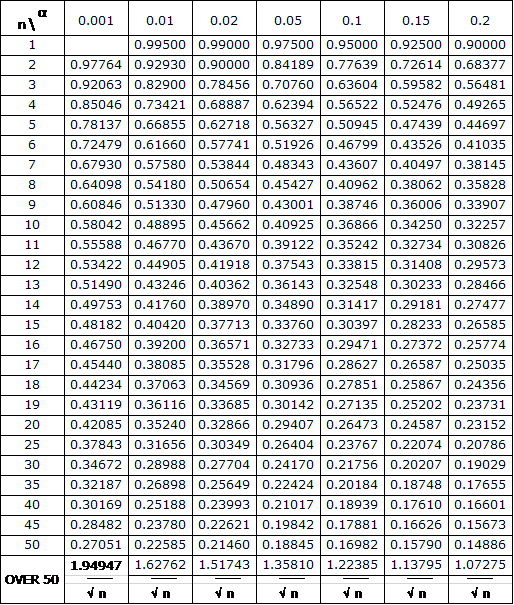
\includegraphics[height=0.5\textheight, angle=0]{"pdf/tablicaK.png"}
\end{center} \end{figure}

\end{document}